\documentclass[10pt]{article}

\usepackage{float}
\usepackage{fullpage}
\usepackage{parskip}

\usepackage{mathtools}
\usepackage{amssymb}
\usepackage{slashed}

\usepackage{fancyhdr}
\usepackage{array}
\usepackage[margin=0.9in]{geometry}
\usepackage{graphicx}

\setlength{\pdfpagewidth}{8.5in}
\setlength{\pdfpageheight}{11.0in}

\newcommand{\rs}{\sqrt{s}}

\newcommand{\psibar}{\overline{\psi}}
\newcommand{\ubar}{\overline{u}}
\newcommand{\vbar}{\overline{v}}

\newcommand{\order}[1]{\mathcal{O}({#1})}
\newcommand{\paren}[1]{ \left( {#1} \right) }
\newcommand{\bracket}[1]{ \left[ {#1} \right] }

\newcommand{\intdfx}{ \int \! d^4 x }
\newcommand{\intdfy}{ \int \! d^4 y }
\newcommand{\intdfz}{ \int \! d^4 z }

\newcommand{\intdfk}{ \int \! \frac{ d^4 k}{(2\pi)^d} }
\newcommand{\intdfl}{ \int \! \frac{ d^4 l}{(2\pi)^d} }
\newcommand{\intdfq}{ \int \! \frac{ d^4 q}{(2\pi)^d} }

\newcommand{\intddx}{ \int \! d^d x }
\newcommand{\intddy}{ \int \! d^d y }
\newcommand{\intddz}{ \int \! d^d z }

\newcommand{\intddk}{ \int \!  \frac{ d^d k}{(2\pi)^d} }
\newcommand{\intddkE}{ \int \! \frac{ d^d k_E}{(2\pi)^d} }
\newcommand{\intddl}{ \int \!  \frac{ d^d l}{(2\pi)^d} }
\newcommand{\intddlE}{ \int \! \frac{ d^d l_E}{(2\pi)^d} }
\newcommand{\intddq}{ \int \!  \frac{ d^d q}{(2\pi)^d} }
\newcommand{\intddqE}{ \int \! \frac{ d^d q_E}{(2\pi)^d} }

\newcommand{\DeltaNaught}{\sqrt{\beta_1^2-4\beta_0\beta_2} }
\newcommand{\DeltaNaughtSqr}{\beta_1^2-4\beta_0\beta_2 }

\begin{document}
\pagestyle{fancy}
%\pagenumbering{gobble}

\begin{center}
\Large{Integrating the QCD beta function: A letter to the QCDSF Collaboration} \\
\vspace{0.7cm}
\large{Matthew Inglis-Whalen, University of Edinburgh, United Kingdom}
\end{center}

\section*{An inconsistency}

In QCD, the beta function is of central importance to understanding how the theory's gauge coupling 
parameter $g$ depends on an energy scale $\mu$. The beta function is defined as

\begin{equation} \label{eq:beta_def_g} \begin{aligned}
\frac{\partial g(\mu)}{\partial \ln \mu} = -g^3\sum\limits_{k=0}^{\infty} b_k g^k(\mu) \equiv \beta(g(\mu)),
\end{aligned} \end{equation}

with the first four of these coefficients known in the $\overline{MS}$ scheme \cite{vanRitbergen:1997va,Czakon:2004bu}. According to 
the QCDSF Collaboration \cite{Booth:2001qp,Booth:2001uy,Gockeler:2004ad,Gockeler:2004wp,Gockeler:2005rv} and a recent lattice review 
\cite{Aoki:2013ldr}, this differential equation can be solved by the equation

\begin{equation} \label{eq:beta_integ_g} \begin{aligned}
\frac{\mu}{\Lambda}=\exp\paren{\frac{1}{2 b_0 g^2}}\paren{\kappa g^2}^{\frac{b_1}{2b_0^2}}
\exp\bracket{\int_{\tau}^{g} dg' \paren{\frac{1}{\beta(g')}+\frac{1}{b_0 g'^3}-\frac{b_1}{b_0^2 g'}}}.
\end{aligned} \end{equation}

Both QCDSF and the lattice review use $\kappa=b_0$ and $\tau=0$, though these parameters are arbitrary if the sole requirement is for
eq. (\ref{eq:beta_integ_g}) to satisfy eq. (\ref{eq:beta_def_g}). That is to say, $\kappa$ and $\tau$ are determined by internal consistency
relations and by the boundary conditions imposed upon the solution. This arbitrariness may easily be seen by first taking the natural logarithm 
of eq. (\ref{eq:beta_integ_g}) then differentiating both sides with respect to $g$. Cancellations occur entirely independently of the 
parameters $\kappa$ and $\tau$, and the reciprocal of eq. (\ref{eq:beta_def_g}) is recovered.

The goal of this letter is to establish a concrete method of determining these parameters $\kappa$ and $\tau$. In regards to $\tau$, this goal is 
best achieved by first taking the natural logarithm of (\ref{eq:beta_integ_g}) 

\begin{equation} \label{eq:ln_beta_integ_g} \begin{aligned}
\ln \frac{\mu}{\Lambda}=\frac{1}{2 b_0 g^2} + \frac{b_1}{2b_0^2}\ln \kappa g^2 +
\int_{\tau}^{g} \! dg' \paren{\frac{1}{\beta(g')}+\frac{1}{b_0 g'^3}-\frac{b_1}{b_0^2 g'}},
\end{aligned} \end{equation}

then differentiating with respect to $\tau$ and rearranging,

\begin{equation} \label{eq:beta_integ_diff} \begin{aligned}
\frac{1}{\beta(\tau)}&= -\frac{1}{b_0\tau^3}+\frac{b_1}{b_0^2 \tau}.
\end{aligned} \end{equation}

Expanding the reciprocal of the beta function about $\tau=0$ correctly reproduces the right hand side of eq. (\ref{eq:beta_integ_diff}) 
up to $\order{\tau}$ corrections. For consistency, the $\order{\tau}$ corrections must vanish, which implies that $\tau \rightarrow 0$, as given by QCDSF.

To determine $\kappa$, the strategy is to solve for $\ln(\mu / \Lambda)$ using two different methods. The first method involves directly evaluating
the integral in eq. (\ref{eq:beta_integ_g}), while the second method involves integrating eq. (\ref{eq:beta_def_g}) using the boundary condition
$g(\Lambda) \rightarrow \infty$. For both methods, the beta function will be truncated to its two loop form, $\beta(g) = -b_1 g^3(\frac{b_0}{b_1}+g^2)$. This is for the sake of clarity -- the method will work for higher orders in the perturbative expansion, as should be made clear in the
following section.

Both methods require the reciprocal of the beta function to be integrated, which can be achieved using the partial fraction decomposition,

\begin{equation} \label{eq:partial_fractions_g} \begin{aligned}
\frac{1}{-b_1 g^3\paren{ \frac{b_0}{b_1}+g^2 } }=\frac{A}{g}+\frac{B}{g^2}+\frac{C}{g^3}
+\frac{gD}{g^2+\frac{b_0}{b_1}} ,
\end{aligned} \end{equation}

where

\begin{equation} \label{eq:partial_fractions_system_soln} \begin{aligned}
A=\frac{b_1}{b_0^2} && ; && B=0 && ; && C=-\frac{1}{b_0} && ; && D=-\frac{b_1}{b_0^2} 
\end{aligned} \end{equation}

Inserting this decomposition now into eq. (\ref{eq:ln_beta_integ_g}) to solve for $\ln(\mu / \Lambda)$, the $A/g$ and $C/g^3$ terms exactly cancel the singular terms, ensuring the integral is finite:

\begin{equation} \label{eq:beta_integ_g_frac} \begin{aligned}
\ln \frac{\mu}{\Lambda}=\frac{1}{2 b_0 g^2}+\frac{b_1}{2b_0^2}\ln\kappa g^2+
\int_{0}^{g} dg' \paren{-\frac{b_1}{b_0^2} \frac{g'}{g'^2+\frac{b_0}{b_1}} }.
\end{aligned} \end{equation}

Once integrated, this gives the final solution for $\ln(\mu / \Lambda)$

\begin{equation} \label{eq:mu_over_lambda} \begin{aligned}
\ln\frac{\mu}{\Lambda}=\frac{1}{2 b_0 g^2} +\ln\paren{ \frac{b_1}{\kappa b_0}+\frac{1}{\kappa g^2} }^{-\frac{b_1}{2b_0^2}}.
\end{aligned} \end{equation}

The second method begins by integrating the definition of the beta function with the boundary conditions $g(\Lambda) \rightarrow \infty$:

\begin{equation} \label{eq:beta_mymethod} \begin{aligned}
\int_{\infty}^{g} \! \frac{dg'}{\beta(g')} = \int_{\Lambda}^{\mu} \! d \ln \mu' = \ln \frac{\mu}{\Lambda}.
\end{aligned} \end{equation}

One might be wary of integrating the beta function over large values of $g$, since the beta function becomes non-perturbative in this region. 
However, from a purely mathematical point of view, the value of the integral is well-defined, so for the physical results to be internally
consistent, eq. (\ref{eq:beta_mymethod}) is necessarily a true statement. Once again using the partial fraction decomposition to evaluate the integral in eq. (\ref{eq:beta_mymethod}),

\begin{equation} \label{eq:mu_over_lambda_mymethod} \begin{aligned}
\int_{\infty}^{g} \! \frac{dg'}{\beta(g')}&=\int_{\infty}^{g} d g' \paren{\frac{b_1}{b_0^2 g'}-\frac{1}{b_0 g'^3}
-\frac{b_1}{b_0^2} \frac{g'}{g'^2+\frac{b_0}{b_1}} } \\
&=\bracket{ \frac{1}{2b_0g'^2}+ \ln \paren{ 1+\frac{b_0}{b_1g'^2}}^{ -\frac{b_1}{2b_0^2} }  } _{\infty}^{g} \\
&= \frac{1}{2b_0g^2}+\ln \paren{ 1+\frac{b_0}{b_1g^2} }^{ -\frac{b_1}{2b_0^2} }
\end{aligned} \end{equation}

Equation (\ref{eq:beta_mymethod}) establishes an equality between equations (\ref{eq:mu_over_lambda}) and (\ref{eq:mu_over_lambda_mymethod}), allowing
$\kappa$ to be determined. Comparing the two equations, the only valid solution is $\kappa=b_1/b_0$, in tension with the QCDSF 
value of $\kappa=b_0$.

\section*{Pushing forward}

When written in terms of the roots of the beta function, the integral in eq. (\ref{eq:beta_integ_g}) can be performed analytically to any finite 
order in perturbation theory. To one loop order, only $b_0$ is non-zero, and the expression for $\mu / \Lambda$ is

\begin{equation} \label{eq:mu_over_lambda_zeroth} \begin{aligned}
\frac{\mu}{\Lambda}=\exp \paren{\frac{1}{2b_0 g^2}}.
\end{aligned} \end{equation}

To higher orders, integration depends on finding the roots of the beta function. If $N$ denotes the index of the last non-vanishing coefficient $b_k$, 
then the beta function can be rewritten in terms of its non-zero roots $r_k$:

\begin{equation} \label{eq:beta_roots} \begin{aligned}
\beta(g)&=-b_N g^3\prod\limits_{k=1}^{N} (g^2-r_k)
\end{aligned} \end{equation}

The partial fraction decomposition for the reciprocal of eq. (\ref{eq:beta_roots}) is

\begin{equation} \label{eq:partial_fraction_N} \begin{aligned}
\frac{1}{-b_N g^3}\prod\limits_{k=1}^{N} \frac{1}{g^2-r_k}=\frac{A}{g}+\frac{B}{g^2}+\frac{C}{g^3}+\sum\limits_{k=1}^{N}\frac{gP_k}{g^2-r_k}
\end{aligned} \end{equation}

with

\begin{equation} \label{eq:partial_fraction_N_coeffs} \begin{aligned}
A&=\frac{(-1)^{N+1}}{b_N}\bracket{\prod\limits_{k=1}^{N}\frac{1}{r_k}}\bracket{\sum\limits_{k=1}^{N} \frac{1}{r_k}} \\
B&=0\\
C&=\frac{(-1)^{N+1}}{b_N}\prod\limits_{k=1}^{N} \frac{1}{r_k}                                                           \\
P_k&=-\frac{1}{b_Nr_k^2}\prod\limits_{\substack{j=1 \\ j \neq k}}^{N} \frac{1}{r_k-r_j}
\end{aligned} \end{equation}

By expanding eq. (\ref{eq:beta_roots}) and collecting powers of $g^2$, it can be shown that the expressions for $A$ and $C$ simplify 
to $A=b_1/b_0^2$ and $C=-1/b_0$. These values for $A$ and $C$ are what allow the singular terms of eq. (\ref{eq:beta_integ_g}) to be exactly
cancelled, regardless of expansion order. Using the values $\kappa=b_1/b_0$ and $\tau=0$ determined in the previous section, the closed form expression 
for $\mu / \Lambda$ is then

\begin{equation} \label{eq:mu_over_lambda_orderN} \begin{aligned}
\frac{\mu}{\Lambda}=\exp \paren{\frac{1}{2b_0 g^2}}\paren{\frac{b_1}{b_0}g^2}^{\frac{b_1}{2b_0^2}}
\prod\limits_{k=1}^{N} \paren{1-\frac{g^2}{r_k}}^{\frac{P_k}{2}}.
\end{aligned} \end{equation}

Equation (\ref{eq:mu_over_lambda_orderN}) holds provided none of the roots $r_k$ are repeated. The nonzero 
roots of the beta function are, in general, complex, but the imaginary component of eq. (\ref{eq:mu_over_lambda_orderN}) vanishes exactly, as it 
must for a purely real integral. One should be aware, however, that computational rounding errors can introduce a small imaginary component when
evaluating the expression numerically. Taking the real part of the result solves any problems that may be connected to this issue. 

No closed form expression exists for the roots of the 6 loop beta function, since this involves solving the quintic. Conversely, however,
eq. (\ref{eq:mu_over_lambda_orderN}) can be fully written down in terms of radicals for any perturbative expansion to 5 loops or less, owing to well
known general solutions of quartic functions. 

Appendix A contains plots comparing analytic solutions to $\mu / \Lambda$ with $\kappa=b_0$ and $\kappa=b_1/b_0$, as well as the numerically inverted solutions for $\alpha(\mu)\equiv g^2(\mu)/4\pi$ up to four loops.

\vspace*{\fill}
 
%The QCD beta function may alternatively be written in terms of the QCD coupling constant $\alpha(\mu)\equiv g^2/4\pi$,
%
%\begin{equation} \label{eq:beta_def_alpha} \begin{aligned}
%\frac{d \alpha(\mu)}{d \mu^2} = -\alpha^2\sum\limits_{k=0}^{\infty} \beta_k\alpha^k(\mu) \equiv \beta(\alpha(\mu)).
%\end{aligned} \end{equation}
%
%A solution similar to eq. (\ref{eq:beta_integ_g}) can be constructed in terms of $\alpha$,
%
%\begin{equation} \label{eq:beta_integ_alpha} \begin{aligned}
%\frac{\mu}{\Lambda}=\exp\paren{\frac{1}{2 \beta_0 \alpha}}\paren{\frac{\beta_1}{\beta_0} \alpha}^{\frac{b_1}{2b_0^2}}
%\exp\bracket{\frac{1}{2}\int_{0}^{\alpha} d\alpha' \paren{\frac{1}{\beta(\alpha')}+\frac{1}{\beta_0 \alpha'^2}-\frac{\beta_1}{\beta_0^2 \alpha'}}}.
%\end{aligned} \end{equation}
%
%This integral can be performed analytically to any finite order in perturbation theory, again through the use of partial fractions. 
%To one loop order,
%
%\begin{equation} \label{eq:beta_integ_1loop} \begin{aligned}
%\frac{\mu}{\Lambda}=\exp\paren{\frac{1}{2\beta_0\alpha }},
%\end{aligned} \end{equation}
%
%while for any number of loops $N_L>1$, 
%
%\begin{equation} \label{eq:beta_integ_NLloop} \begin{aligned}
%\frac{\mu}{\Lambda}=\exp\paren{\frac{A}{2\beta_{N_L-1}\alpha }} \alpha^{\frac{-B}{2\beta_{N_L-1}}} 
%                    \, \prod\limits_{k=1}^{N_L-1} (\alpha-r_k)^{\frac{-P_k}{2\beta_{N_L-1}}}
%\end{aligned} \end{equation}
%
%where $r_k$ are the nonzero roots of the QCD beta function and $A$, $B$, and $P_k$ are the coefficients of the partial fraction
%decomposition,
%
%\begin{equation} \label{eq:partial_fractions} \begin{aligned}
%\frac{1}{\alpha^2}\prod\limits_{k=1}^{N_L-1}\frac{1}{\alpha-r_k}
%=\frac{A}{\alpha^2}+\frac{B}{\alpha}+\sum\limits_{k=1}^{N_L-1} \frac{P_k}{\alpha-r_k}.
%\end{aligned} \end{equation}
%
%In closed form, these coefficients are
%
%\begin{equation} \label{eq:beta_integ_NLloop_constants} \begin{aligned}
%A&=(-1)^{N_L-1}\prod\limits_{k=1}^{N_L-1} \frac{1}{r_k}                                                           \\
%B&=(-1)^{N_L-1}\bracket{\prod\limits_{k=1}^{N_L-1}\frac{1}{r_k}}\bracket{\sum\limits_{k=1}^{N_L-1} \frac{1}{r_k}} \\
%P_k&=\frac{1}{r_k^2}\prod\limits_{\substack{j=1 \\ j \neq k}}^{N_L-1} \frac{1}{r_k-r_j}
%\end{aligned} \end{equation}
%
%Equation (\ref{eq:beta_integ_NLloop}) holds provided none of the roots $r_k$ are repeated; see Appendix A for a proof. The nonzero 
%roots of the beta function are, in general, complex, but the imaginary component of the expression vanishes exactly, as it must for
%a purely real integral. One should be aware, however, that computational rounding errors can introduce a small imaginary component when
%evaluating the expression numerically. Taking the real part of the result solves any problems that may be connected to this issue. 
%
%The form of eq. (\ref{eq:beta_integ_NLloop}) does not invite a closed form inversion to solve for $\alpha(\mu)$. Numerically 
%inverting eq. (\ref{eq:beta_integ_NLloop}) for $2 \leq N_L \leq 4$, Figure \ref{fig:alpha_of_mu_matt} 
%shows the running of the coupling up to the highest order of $\beta_k$ currently known in perturbation theory.
%

\appendix
\section{Appendix A}

\begin{figure}[H]
\begin{center}
  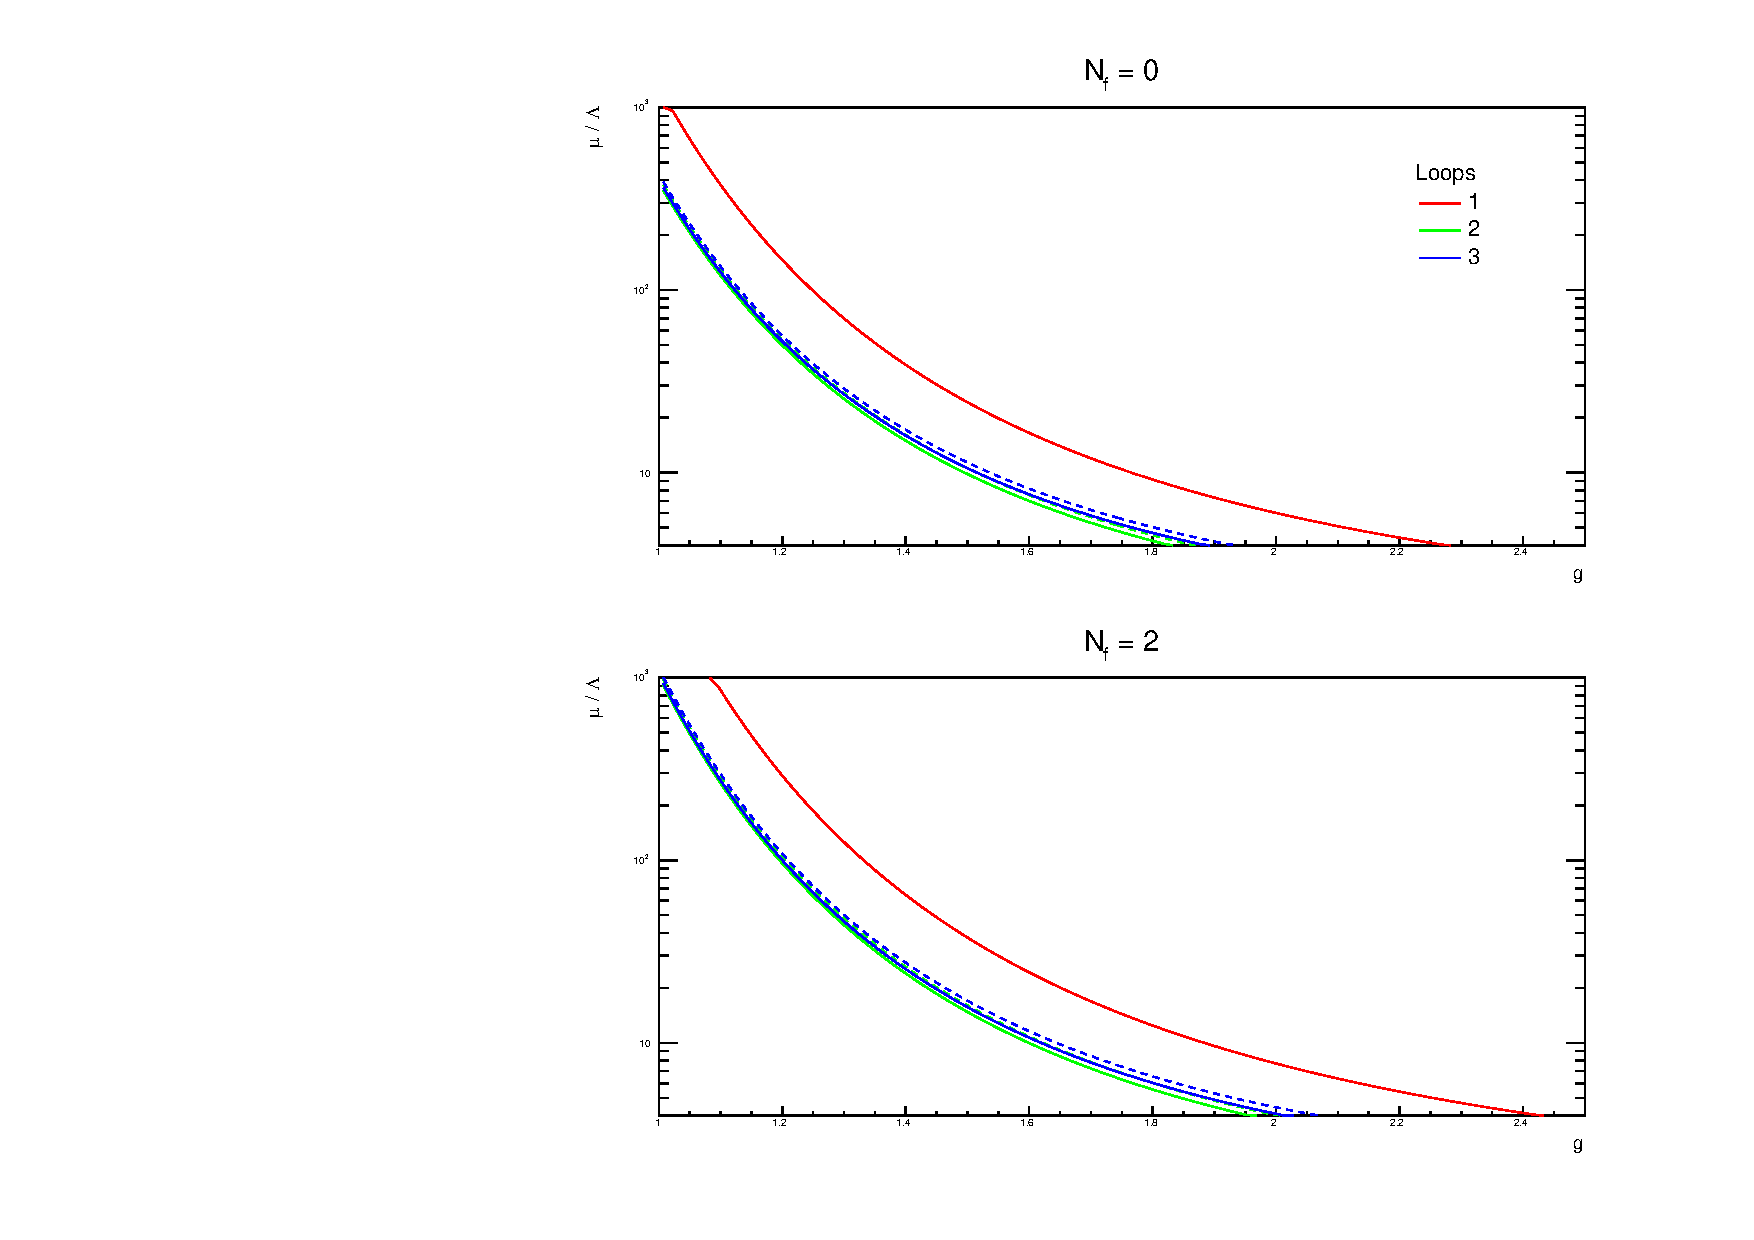
\includegraphics[width=5.0in]{mu_over_lambda_analytic.pdf}
  \caption{$\mu / \Lambda$ vs $g$ in the $\overline{MS}$ renormalization scheme for the quenched approximation (top) and for $n_f=2$ 
(bottom), using increasingly higher orders in the perturbative expansion. $\kappa=b_0$ appears as a dashed line while $\kappa=b_1/b_0$
appears as a solid line. }
  \label{fig:mu_over_lambda_analytic}
\end{center}
\end{figure}

\begin{figure}[H]
\begin{center}
  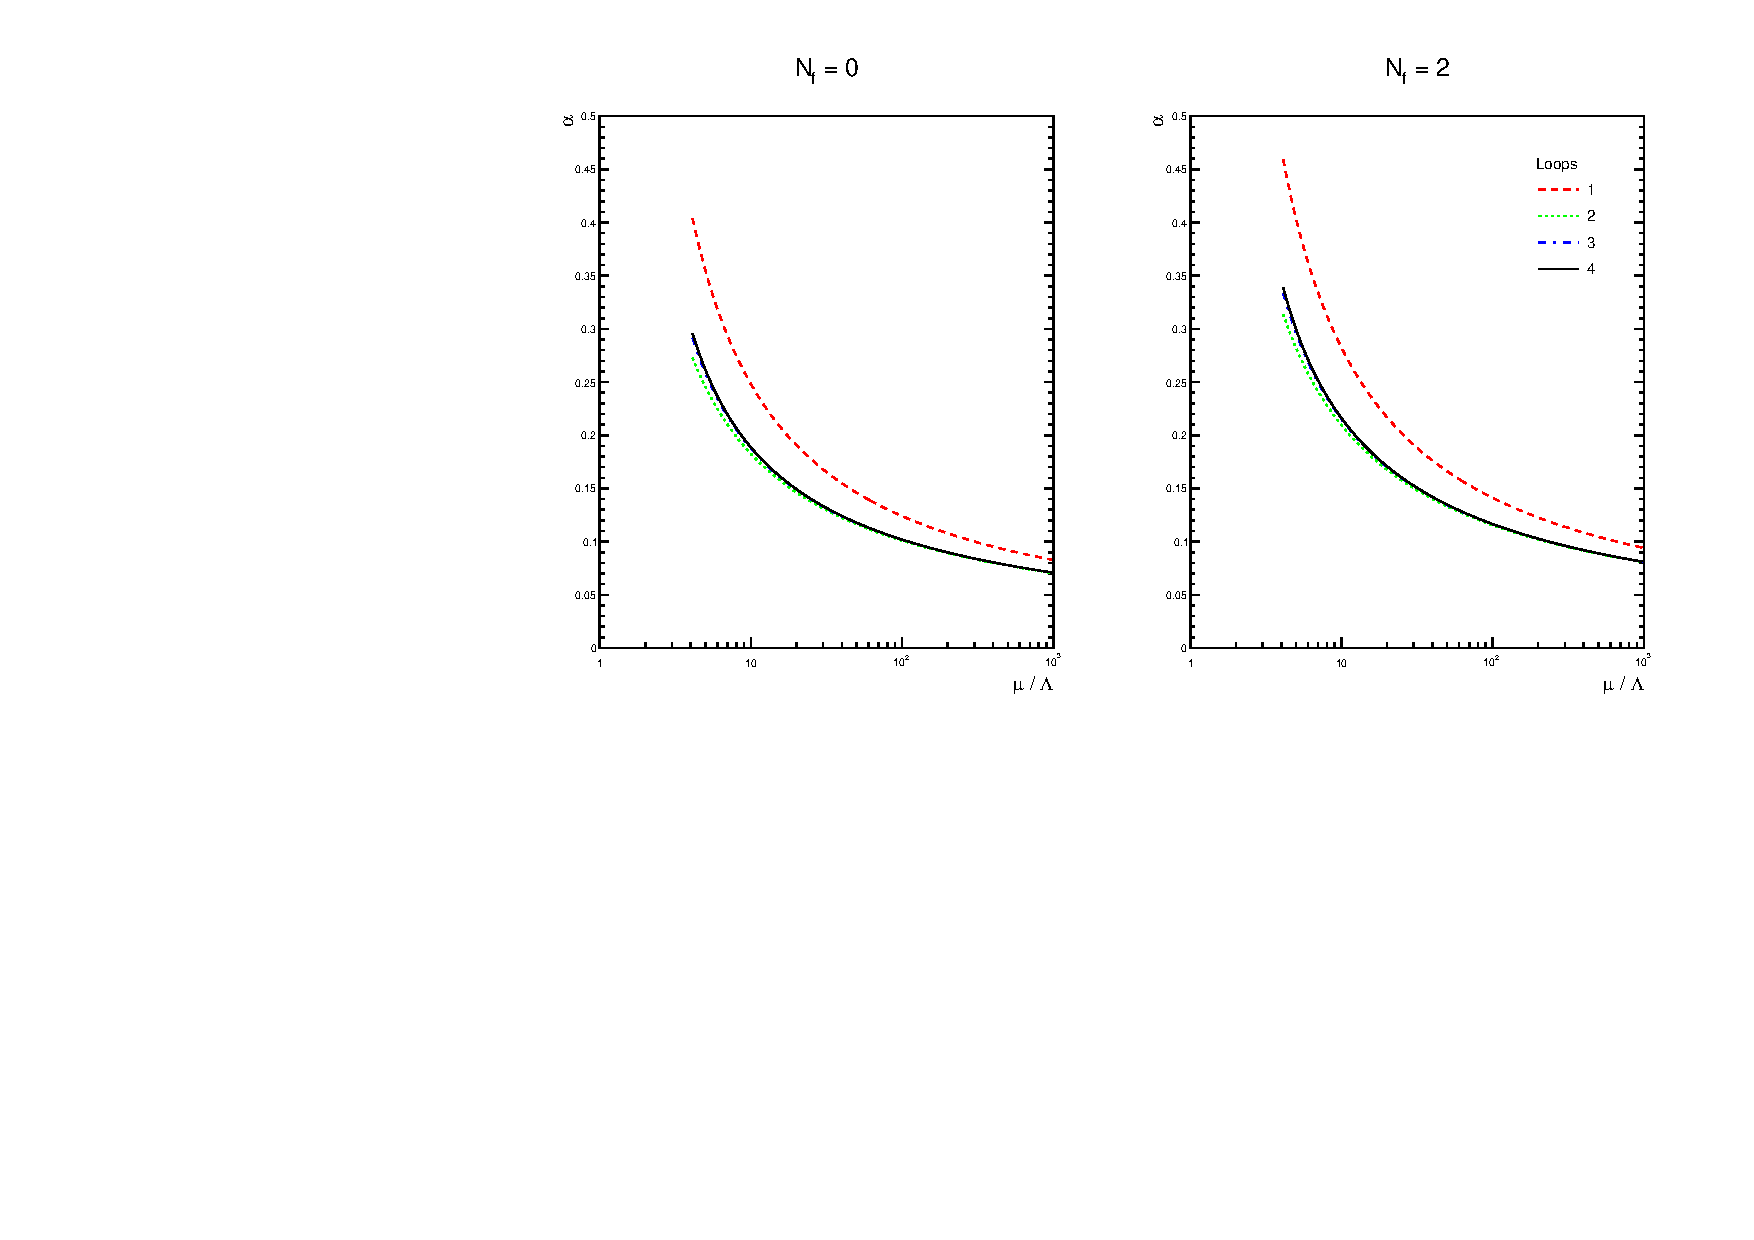
\includegraphics[width=6.5in]{alpha_of_mu_analytic.pdf}
  \caption{$\alpha$ vs $\mu / \Lambda$ in the $\overline{MS}$ renormalization scheme for the quenched approximation (left) and for $n_f=2$ 
(right), using increasingly higher orders in the perturbative expansion, with $\kappa=b_1 / b_0$.}
  \label{fig:alpha_of_mu_analytic}
\end{center}
\end{figure}

\vspace*{\fill}

\begin{thebibliography}{10}

%\cite{vanRitbergen:1997va}
\bibitem{vanRitbergen:1997va}
  T.~van Ritbergen, J.~A.~M.~Vermaseren and S.~A.~Larin,
  %``The Four loop beta function in quantum chromodynamics,''
  Phys.\ Lett.\ B {\bf 400} (1997) 379
  [hep-ph/9701390].
  %%CITATION = HEP-PH/9701390;%%
  %692 citations counted in INSPIRE as of 12 Jun 2014

\bibitem{Czakon:2004bu}
  M.~Czakon,
  %``The Four-loop QCD beta-function and anomalous dimensions,''
  Nucl.\ Phys.\ B {\bf 710} (2005) 485
  [hep-ph/0411261].
  %%CITATION = HEP-PH/0411261;%%
  %198 citations counted in INSPIRE as of 12 Jun 2014

%\cite{Booth:2001qp}
\bibitem{Booth:2001qp}
  S.~Booth {\it et al.}  [QCDSF-UKQCD Collaboration],
  %``Determination of Lambda(MS-bar) from quenched and N(f)=2 dynamical QCD,''
  Phys.\ Lett.\ B {\bf 519} (2001) 229
  [hep-lat/0103023].
  %%CITATION = HEP-LAT/0103023;%%
  %52 citations counted in INSPIRE as of 15 Jun 2014

%\cite{Booth:2001uy}
\bibitem{Booth:2001uy}
  S.~Booth, M.~Gockeler, R.~Horsley, A.~C.~Irving, B.~Joo, S.~Pickles, D.~Pleiter and P.~E.~L.~Rakow {\it et al.},
  %``The Strong coupling constant from lattice QCD with N(f)=2 dynamical quarks,''
  Nucl.\ Phys.\ Proc.\ Suppl.\  {\bf 106} (2002) 308
  [hep-lat/0111006].
  %%CITATION = HEP-LAT/0111006;%%
  %4 citations counted in INSPIRE as of 15 Jun 2014

%\cite{Gockeler:2004ad}
\bibitem{Gockeler:2004ad}
  M.~Gockeler {\it et al.}  [QCDSF and UKQCD Collaborations],
  %``Determination of Lambda in quenched and full QCD: An Update,''
  Nucl.\ Phys.\ Proc.\ Suppl.\  {\bf 140} (2005) 228
  [hep-lat/0409166].
  %%CITATION = HEP-LAT/0409166;%%
  %8 citations counted in INSPIRE as of 15 Jun 2014

%\cite{Gockeler:2004wp}
\bibitem{Gockeler:2004wp}
  M.~Gockeler {\it et al.}  [QCDSF Collaboration],
  %``A Lattice determination of moments of unpolarised nucleon structure functions using improved Wilson fermions,''
  Phys.\ Rev.\ D {\bf 71} (2005) 114511
  [hep-ph/0410187].
  %%CITATION = HEP-PH/0410187;%%
  %53 citations counted in INSPIRE as of 15 Jun 2014

%\cite{Gockeler:2005rv}
\bibitem{Gockeler:2005rv}
  M.~Gockeler, R.~Horsley, A.~C.~Irving, D.~Pleiter, P.~E.~L.~Rakow, G.~Schierholz and H.~Stuben,
  %``A Determination of the Lambda parameter from full lattice QCD,''
  Phys.\ Rev.\ D {\bf 73} (2006) 014513
  [hep-ph/0502212].
  %%CITATION = HEP-PH/0502212;%%
  %100 citations counted in INSPIRE as of 15 Jun 2014

%\cite{Aoki:2013ldr}
\bibitem{Aoki:2013ldr}
  S.~Aoki, Y.~Aoki, C.~Bernard, T.~Blum, G.~Colangelo, M.~Della Morte, S.~D�rr and A.~X.~El Khadra {\it et al.},
  %``Review of lattice results concerning low energy particle physics,''
  arXiv:1310.8555 [hep-lat].
  %%CITATION = ARXIV:1310.8555;%%
  %64 citations counted in INSPIRE as of 15 Jun 2014

\end{thebibliography}

\end{document}
